% Created 2013-03-04 Mon 11:44
\documentclass[11pt]{article}
\usepackage[latin1]{inputenc}
\usepackage[T1]{fontenc}
\usepackage{fixltx2e}
\usepackage{graphicx}
\usepackage{longtable}
\usepackage{float}
\usepackage{wrapfig}
\usepackage{soul}
\usepackage{textcomp}
\usepackage{marvosym}
\usepackage{wasysym}
\usepackage{latexsym}
\usepackage{amssymb}
\usepackage{hyperref}
\tolerance=1000
\usepackage{baskervald}
\providecommand{\alert}[1]{\textbf{#1}}

\title{Git Quickstart}
\author{Scott Jackson}
\date{Last updated: \today}
\hypersetup{
  pdfkeywords={},
  pdfsubject={},
  pdfcreator={Emacs Org-mode version 7.8.11}}

\begin{document}

\maketitle



\section{Overview}
\label{sec-1}

\begin{description}
\item[What's in this tutorial?] This takes you through all of the basic commands you need to get started using git right away. You will learn:
\begin{enumerate}
\item How to start tracking a project with git.
\item How to commit changes to a project.
\item How to manage files with git.
\item How to look at the history of commits.
\item How to ``rewind the tape'' on a project.
\item How to customize your setup.
\end{enumerate}
\item[What do I need to start?] You need a computer and the ability to install software on it. I will briefly address installation.  If you have never worked with a command-line program before, then I highly recommend going to my miscellaneous tutorial on \href{https://github.com/shoestringpsycholing/rrr_tools/misc_tutorials/}{using the command line}.
\item[How long will this take?] Once you have things installed, you should be able to get through this entire tutorial in about an hour.
\end{description}
\section{Installation}
\label{sec-2}

Installation should be a breeze. Just go to \href{http://git-scm.com}{the main git website}, and follow the links for downloads, and select the operating system you have.

\textbf{NOTE ON WINDOWS}: Windows has a very sad little command-line program called \texttt{cmd.exe}. You can start one by typing ``cmd'' in the Start menu search bar (if you're in Windows 7), or in the ``Run\ldots{}'' field in the start bar in earlier versions of Windows. The problem is that git needs some utilities that are not provided by this basic Windows interface, so you have to make some choices during installation. You can pretty much just select the default options it gives you, but then you are faced with a three-way choice:
\begin{description}
\item[Use Git Bash only] The installer tells you this is the ``most conservative choice.'' Basically this leaves everything alone with the default Windows command line, and installs a special command line program called the ``Git Bash.''\footnote{''Bash'' stands for \href{http://en.wikipedia.org/wiki/Bash_(Unix_shell)}{Bourne-again shell}, and is a popular and common command-line interface originally for Unix systems.
 } This basically means that git commands will only work in the Git Bash, not in your default command prompt.  Especially if you are just starting out with git, I recommend this, since it's the most ``lightweight'' option.
\item[Run Git from the Windows Command prompt] If you have reason or interest in installing an alternative command-line program such as \href{http://www.cygwin.com/}{Cygwin}, you may want this option. Cygwin basically gives you a Unix-style command-line program, including a bunch of other (optional) tools. If you have Cygwin installed, selecting this option means that you can run git from a Cygwin shell.  If you don't have Cygwin (or something similar) installed, don't bother.
\item[Run Git and included Unix tools from the Windows Command Prompt] This option comes with a warning that you should do this ``only if you understand the implications.'' Personally, I don't see the point, unless you know enough about the other tools of the standard Windows command-line that you know you don't need a bunch of them.
\end{description}

You may also need to make a decision about ``line endings.'' In a nutshell, different operating systems (like Windows and Mac) use different symbols to represent the end of a line in a text file (don't ask me why!). The installer makes recommendations, in order to help manage cross-platform projects.  I recommend you follow the recommendations!\footnote{In Windows, the top option ``Checkout Windows-style, commit Unix-style line endings'' is recommended. Because Mac is based on Unix, I assume the second option (``Checkout as-is, commit Unix-style line endings'') is preferred on Mac (and Linux), but if you know better, let me know!
 }

When installation is complete, you should be able to open up a command line program (in Windows, either the Git Bash or a Cygwin Bash), type in \texttt{git version}, and have it tell you the version number of git that you have installed. If you get a message saying that a program called ``git'' doesn't exist, then the installation didn't quite go right.
\section{Initial set-up}
\label{sec-3}

There's one last step you need to do after installing git, and that's tell it who you are.  We'll see later how this comes into play. For now, just start the command-line program where you can run git, and type in the two following lines, substituting your information instead of mine (note the double-dash before \texttt{global}):


\begin{verbatim}
git config --global user.name "Scott Jackson"
git config --global user.email shoestringpsycholing1@gmail.com
\end{verbatim}

By using the \texttt{-{}-global} option, these settings will be kept for all of your interactions with git on this computer. You can always change these later, but you need to set them before you can proceed with the tutorial.
\section{Interacting with git}
\label{sec-4}

If you have browsed around the git site, or if you've seen git in other places, you may have seen graphical interfaces (GUIs) advertised.  I recommend you \emph{avoid} those, especially if you are just starting out. If you are still new to the command line and have some anxiety about it, please check out my tutorial on the command line in the miscellaneous tutorials section.

Why stick with the command line? As you will see shortly, the everyday git commands are very simple. One of the advantages of git is its speed, because this allows you to commit frequently, commit liberally, branch whenever you feel like it, and so on, without disrupting your workflow. It will take you a couple of tries to remember some of the commands, but you can do most things with eight or so commands, which is not too much of a memory burden.  Especially if you print out the reference card that accompanies this tutorial, it's not a big deal.  Dealing with a GUI, on the other hand always takes longer, and is just a lot more involved. Plus, the GUI is more likely to change over time, and this hurts reproducibility. So unless you get into some really complex branching situations where a visualization of the history is super-handy, I highly recommend avoiding any of the git GUIs, and just sticking with the command line.

So here's a basic example of how you might interact with git in a normal day of work:
\begin{enumerate}
\item Decide what project you want to work on for the moment.
\item Start a command line program that can run git.
\item (Assuming the project is already being tracked in git) Run \texttt{git status} to check on whether you have any untracked changes or anything else you need to clean up.
\item Do your work!
\item When you hit some kind of stopping point, run \texttt{git status} again to remind yourself what files you worked on, added, removed, or modified.
\item Decide if you want to include all these changes in one snapshot, or if you want to break them up.
\item Use \texttt{git add} and \texttt{git rm} commands to prepare (or ``stage'') the snapshot.
\item Use \texttt{git commit} to commit the changes to the project history, and give a brief message about what the changes were.
\item Rinse and repeat!
\end{enumerate}

This looks like a lot of steps, but it's the steps 5 through 8 that you'll do over and over, and they take about a minute or less, depending on how detailed you want to make the commit message.  But the basic idea is that you have some kind of command-line program open while you do your work, so when it's time to commit changes, you just pop over, type a line or two, and pop back to your work.\footnote{And if you're working in Emacs, you can run the command-line shell within Emacs, so you don't even need to leave Emacs to use git.
 } The point is to keep your interaction with git unobtrusive and not distracting from your real work!

Now let's dive into the details, so you can start using it yourself.
\section{Start tracking with \texttt{git init}}
\label{sec-5}

I suggest you follow along with this tutorial as we go. The first step is to start a command line where you can run git.  If can type \texttt{git version}, hit Enter/Return, and get a version number back, you're all set.

Now, it's time to create a project that you want to track.  I \emph{highly} recommend starting a fresh new folder instead of starting with a folder with a lot of important files already in it.  For the purposes of this tutorial, we'll just call the folder ``gitplay''.

Next, you need to navigate your command line to this new folder.  Depending on how you installed git, you may have the option to right-click (or control-click in Mac) and select ``Git Bash here'' to start a command line in that folder right away. If you need to brush up on the basics of changing directories in the command line, check out my brief tutorial on the command line in the miscellaneous section.

Now, all you need to do to start tracking that folder (and all of its contents, including subfolders) is to type this at the prompt and hit Return:


\begin{verbatim}
git init
\end{verbatim}

Now this folder is called a \emph{repository} (or \emph{repo}) in git lingo.  Congrats, it's your first git repository!\footnote{If you have the option on to ``show hidden folders'' in your operating system, you may see a folder called ``.git'' appear in your repo. This is actually where all the information is stored that git uses to track your changes. So you should leave it alone!  You can delete this folder the normal way, but this will obliterate all of the history that git tracked in your project, kind of like a ``clear history'' in your web browser deletes all of your browsing history.
 }
\section{Using \texttt{git add} and \texttt{git commit} to take snapshots}
\label{sec-6}

Next, you should put a file in the folder. In can be any kind of file.  For example purposes, let's say you have a text file called \texttt{mytext.txt}.  Put it in the folder, and run the command:


\begin{verbatim}
git status
\end{verbatim}

This is a handy command that I use very frequently. It will tell you a number of things, but in this case it will tell you that you have an ``untracked'' file called \texttt{mytext.txt}, and it will (perhaps helpfully) remind you that you use \texttt{git add} to start tracking a file.  Let's do that next!  Type this (assuming you're playing along and added a file called \texttt{mytext.txt}):


\begin{verbatim}
git add mytext.txt
\end{verbatim}

Git won't tell you anything in response, but this file has now been \emph{staged}. Run \texttt{git status} again, and it will reflect this change.  Note that it now says that there are ``changes \emph{to be} committed.''  In other words, the changes are not committed yet! Here's a sketch of how this works.



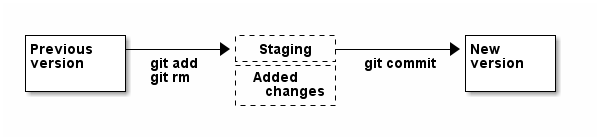
\includegraphics[width=.9\linewidth]{commitflow1.png}

So by using \texttt{git add}, you've told git to add the new file to the staging area, and then the next time you run \texttt{git commit}, it takes everything in the staging area and adds it to the new version of your project.  Let's do that now:


\begin{verbatim}
git commit -m "first commit, added mytext"
\end{verbatim}

Now if you run \texttt{git status} again, it will tell you ``nothing to commit, working directory clean''.  Congratulations, you have performed your first commit!  This is the starting point in the history of this new repo. 

Now, let's go back and unpack that last command a bit. The \texttt{git commit} is the basic command, and the \texttt{-m} part is an \emph{option}. It's a little flag that tells git ``hey, I want to turn on an option for this command, just this time.''  The option this turns on is the ``message'' option. As I mentioned, every time you add a snapshot to the history of your project/repository, you should add some annotation or notes to say something about what changes you made. If you have just something short to add, using this option lets you just type out the message in quotes as part of the \texttt{git commit} command.  This is a nice, speedy way to add a short note.  If you leave off this flag, git will open up a text editor, where you can write out as long or as short a message as you'd like.  Then when you save and close the editor, git uses that message for the commit, and finishes the commit.  So there are several ways to enter the message for your commit, and you can pick the one that you like, but the bigger point here is that git commands often have many different options you can use to make it work better for you.

The next step in your workflow is just to keep working!  So let's say we need to make some changes to \texttt{mytext.txt}.  Go ahead and make some changes, by adding and/or deleting some text. Git is not ``doing'' anything while you're working. It's just waiting in the background for you to tell it what to do next.  So work on the file as you would normally work on it.

Now let's assume you get to some kind of stopping point.  Time to commit these changes to the history!  First, run \texttt{git status}.  Notice that now git tells you that this file has been modified, which was different from the initial feedback we got, which was that this file was ``untracked.'' Git helps you keep track of which files have just been updated vs. those that were added completely new.  Git also gives you a couple of tips/reminders for some things you might want to do, like add these changes to the staging area with \texttt{git add}, or discarding the changes you made with \texttt{git checkout}.  Let's not worry about the latter now, but adding these changes to the history is what we want, so let's do that.  This time, let's take a little shortcut:


\begin{verbatim}
git add .
git commit -m "updated mytext.txt"
\end{verbatim}

When git is expecting a file name, like \texttt{git add <filename>}, you can actually pass it a lot of different things to make your life easier.  The period (\texttt{.}) means ``everything in this directory.''  This is handy because many times, you'll work on several different files in your project, and you know that you just want git to add all the changes to the next commit.  Using \texttt{git add .} is an easy way to do that.  And again, we used the \texttt{-m} option with \texttt{git commit} to add a short message.

Let's do this one more time, and I'll show you another shortcut. So make some more changes to \texttt{mytext.txt}.  When you're done (and you saved those changes normally in your editor), run the following:


\begin{verbatim}
git commit -a -m "updated mytext.txt some more"
\end{verbatim}

Another option! The \texttt{-a} option tells git to first \texttt{add} everything \emph{that is already being tracked}, and then commit those changes.  This is another way to streamline things a bit.  So if you are working a lot on the same files over and over, and are not adding any new files, this is a convenient way to update the history of your repo with a single command, so you can get back to work with minimal interruption.  So now we have several ways to add changes, by using \texttt{git add} with a filename to add things individually, \texttt{git add .} to add all changes all at once, and \texttt{git commit -a}, which rolls adding into the commit command.  Use what feels comfortable to you; the point is that git gives you lots of different ways to go about the process of taking snapshots and tracking your changes over the history of the project.
\section{Using \texttt{git rm} and \texttt{git mv} to manage files}
\label{sec-7}

When git is tracking a folder as a repository, it's not only tracking the contents of the files, but also what files are coming and going, what files are named, and so on. You can use whatever means you normally do to move/rename/delete files, but sometimes doing that within git can be more convenient and easier to deal with.

Let's make a copy of the \texttt{mytext.txt} file, and call it \texttt{mytextcopy.txt}.  Do this in whatever way you are accustomed.  Now let's add and commit that change:


\begin{verbatim}
git add .
git commit -m "added copy of mytext"
\end{verbatim}

What happens if we delete this file?  Go ahead and delete it by dragging the file to the trash, or however you normally delete stuff.  Now run \texttt{git status} to see what git thinks of this.  In fact, it tells us that this file was deleted, but that this change is not yet committed.  Let that sink in a second.  We just threw a file away, but git hasn't committed the change.  Let's follow the advice that the status message gives us and use \texttt{git checkout -{}- <file>} to discard the changes.  Run the following, and watch what happens in your folder:


\begin{verbatim}
git checkout -- mytextcopy.txt
\end{verbatim}

The file is back! Neat! We just used git to hit the ``Undo'' button on the changes to that file, even though the ``changes'' were complete deletion. This is very cool. So how do we actually delete files?  Ultimately, in order to update the history of our project with that deletion, we need to use the \texttt{git rm} command. Run these commands, and watch your folder:


\begin{verbatim}
git rm mytextcopy.txt
git status
git commit -m "deleted the extraneous copy of mytext"
\end{verbatim}

Notice the first command did the deletion for us, as well as adding that change to the staging area. The status message confirms that the deletion will be committed in the next commit.

But what if we realize later that we really needed that file?  Remember that all of the changes up to this point are just part of the history, so we can ``rewind'' to an earlier point, before the deletion, and find the file completely intact, just as it was.  We will go over how to do that a little later.  The point here is that git gives you a big giant safety net for every change that you commit, so if you ever do anything you later regret, as long as it was committed as a snapshot to your history, you can recover it!
\section{Using \texttt{git log} to look at the history}
\label{sec-8}

Speaking of history, we've build up some history to this little toy project already, so let's look at how to inspect that history.  Try this:


\begin{verbatim}
git log
\end{verbatim}

We get a lot of information back!  As you can see, the basic structure is:


\begin{verbatim}
commit bighairylongstringofnumbersandletters
Author: Your Name <email@mail.com>
Date: Date and time, with time zone info

    commit message
\end{verbatim}

I'll go through each of these:

\begin{description}
\item[bighairylongstring\ldots{}] This is the \emph{hash} code for that particular snapshot in the sequence. Hash codes are interesting in their own right, but all you really need to remember is that this long code is the unique code that designates that particular snapshot in your history, with all the files and folders and their contents that were part of that snapshot.  Whenever you need to refer to a particular point in your history, you do so with this thing.  Usually you can get away with just entering in the first few characters, just to the point that it's not ambiguous with any other hash in your history.  So don't worry, you rarely if ever will have to type out this whole thing.
\item[Author] This is the name and email you provided during set-up using \texttt{git config}. This information is just as much part of the snapshot as all the file contents. It tells everyone who made the commit. This is an interesting feature, because you can use it to track who contributed what, if you are using git to collaborate.  More on that in another tutorial.
\item[Date] The exact time and date of the commit, which can also be very handy if you ever need to reconstruct what you did and when.
\item[commit message] Now you can see how helpful a good commit message can be!  A nice, clear commit message can really help you navigate and make sense of the project history. It's up to you how succinct or verbose you want to be, since both have their pros and cons.  I think I personally try to keep them short, because this allows me to update quickly and not get too sidetracked with the process of committing changes, and since you can always ``rewind'' to that point, you can always dig around more in-depth if you need to.  But sometimes, if you make a particularly important change, you may want to describe more about what you did than ``updated file.''  It's up to you!
\end{description}

There are lots of ways to get more or less detailed information from \texttt{git log}, but I'll deal with that in another tutorial. The point here is that \texttt{git log} gives you a history of your ``tracked changes.''

\textbf{INTERFACE TIP}: Depending on how your command-line program works, commands like \texttt{git log} may give you enough output that it has to scroll past the size of the window. You can keep hitting Enter/Return to scroll down one line at a time, or you can hit the spacebar to scroll to the end, and when you're at the end, you may see \texttt{(END)} with a highlighted background. At \emph{any point} in this scrolling interface, you can hit the ``q'' key to ``quit'' and return to the normal command-line prompt.  Being a relative novice with \texttt{bash} myself, this took me far too long to figure out.  If you ever get really stuck with the interface, you can always just close it out and start a new shell. The shell is just a way to run commands, there's nothing else you need to ``save'' for the purposes of using git. So close the shell window whenever you need to, and rest easy that won't affect your git history at all.
\section{Using \texttt{git checkout} to move around in the history}
\label{sec-9}

Now that we can see the history with log, let's play around with the ``rewind'' function. Recall that in the last commit, we deleted the copy of our little text file. Let's imagine that this was a bad idea, and we want to rewind back to the stage where that file was still in our folder. In my version of this project, I can do this with the following:


\begin{verbatim}
git checkout 675f43
\end{verbatim}

Here's how this works. I can look at the log, and see that I have a commit with the message ``deleted the extraneous copy of mytext.''  And I can see that the commit one earlier than that says ``added copy of mytext.'' So I know that's where I want to rewind it to.  So all I need to do is tell git that this is the one, and I can do that by identifying it with the hash.  I don't want to type out the whole hash, so I just type the first several characters (that's the \texttt{675f43} part).  Yours will be different, because your commit will have different contents.

When you do this, git gives you a big warning about how you are in `detached HEAD' state. I will explain this in another tutorial. The point here is that since we haven't made a special branch for this part of the history, anything we do to this part of the history is basically temporary in terms of our repo history.  If you did this successfully, you'll see that the \texttt{mytextcopy.txt} has come back into the folder!  If you wanted to keep that file, one way to do it would be to just copy the file into some other folder (outside the \texttt{gitplay} repo), and then tell git to return back to our ``present state'' of this repo with:


\begin{verbatim}
git checkout master
\end{verbatim}

By default, the main branch of your repo is always called \texttt{master}. So by doing \texttt{git checkout master}, you basically just use the time machine to go back to the ``present day.'' The \texttt{mytextcopy.txt} file will disappear again, the other contents and files that were added or removed will go back to what they were, etc.  But if you copied that old file into some other folder, that copy is left alone.  That is, git seems like it's doing some magic here, but the domain of the magic is the repository.  It can't touch anything outside the repository.

In later tutorials, I will go through more sophisticated ways to recover older versions of your files, but this method is an easy and powerful way to quickly (and temporarily) ``rewind'' a project to an earlier state, grab a file or whatever you needed from that earlier time, and then hop back to the current version with \texttt{git checkout master}.
\section{Customizing your setup}
\label{sec-10}

Congratulations! At this point you have learned pretty much everything you need to know in order to use git as a universal ``track changes'' setting, ``undo'' button, and as a general magic time machine for any of your projects.  Getting in the habit of frequently committing changes and adding messages to describe what you're doing lays a very strong foundation for producing reproducible research, because you are creating a fully ``re-playable'' history of your entire project!  No other tool gives you such extensive reproducibility as a good version control system, and git is one of the best out there. There are plenty of other ways to get similar effects, and plenty of other software tools to do version control, but following the guidelines here will get you a lot of value with very little overhead.

After you have been using git for a while, you may want to further customize it for your needs.  There are \emph{lots} of ways to do this, but I will touch on a few of the easiest and handiest here.
\subsection{\texttt{.gitignore}}
\label{sec-10-1}

Sometimes there are certain kinds of files that you just don't care about.  If you start using Emacs, you'll find that Emacs backs up files regularly, by creating files with the same filename, followed by a tilde (\texttt{\textasciitilde{}}) symbol. If you start using \LaTeX{}, you'll find that processing a \LaTeX{} file into a PDF produces a bunch of files that are basically temporary files, which you don't need once you have a PDF.  One example is files that end with \texttt{.aux}.  If I use git to track changes, I will either have to constantly add these files, which I don't care about, or I'll have to constantly ignore them when \texttt{git status} reminds me that I'm not tracking them.  A much more convenient solution is to use a \texttt{.gitignore} file.  

Here's how that works. You just go to the top folder in the repo, and add a text file with the name \texttt{.gitignore}.  Depending on what text editor you're using, you may need to make sure you're not creating \texttt{.gitignore.txt} or something like that.  Inside the \texttt{.gitignore} file, you add a line for each kind of file you want to ignore.  In addition to the two examples above, let's say I have a bunch of files that I want to keep around in the folder, but I don't want to track. Let's say I make a folder called ``junk'' and I keep all the files I want git to ignore in there.  I could then make my \texttt{.gitignore} file look like this (hitting return after each line):


\begin{verbatim}
*~
*.aux
junk/
\end{verbatim}

The asterisk is a ``wildcard'' character, so the first line says ``anything that ends with a tilde.''  The second line means ``anything that ends with .aux''. And the third line says ``the folder called junk (and all its contents)''.  All of the files matching these descriptions will be completely invisible to git. This is a very flexible and powerful way to keep your git repos clean and to simplify your processes of adding and tracking files.  You can also name particular files, if there's some reason there are specific files that you want to keep around but always ignore.
\subsection{\texttt{git config}}
\label{sec-10-2}

In the beginning, we used \texttt{git config} to set up your name and email, because git uses that information when making commits. But there are lots of other things you can set with \texttt{git config}, so you may want to check out the help on it, to see if anything would make your life easier.  Personally, I like to use Emacs to edit text, and you can do the same if you run the following command:


\begin{verbatim}
git config --global core.editor emacs -q
\end{verbatim}

The string following \texttt{core.editor} is basically the command-line command that starts the editor. I have some fancy start-up options enabled in my regular Emacs, and I don't want those loading when I just want to type out a commit message, so I use the \texttt{-q} option, which tells Emacs to open up without loading any of that.  If your favorite text editor has options like this, you can use them in the same way.  Now, if I run \texttt{git commit} without the \texttt{-m} option, it will open up Emacs (in this minimalist way) so I can type out a more complex message, and then when I save and close that session of Emacs, git uses the message I composed to complete the commit.  This is just one example of an easy way to make git fit in better with your personal preferences. I will probably address many more in other tutorials.
\section{Summary and reference card}
\label{sec-11}

Git is a powerful tool for reproducible research, providing a kind of magic time machine that allows you to visit any point in the history of your repository. This tutorial covered all of the basic commands you need in order to create snapshots of the files and folders in your repository and commit them to the history. Here's a quick summary of the commands. These are also found in the ``reference card'' file that goes along with this tutorial.

\begin{description}
\item[\texttt{git init}] Start tracking changes in a folder (and all its subfolders) by ``initializing'' it as a git repository.
\item[\texttt{git add <file>}] Add a file (or changes to a file) to the set of changes that will be included in the next commit you make (aka the ``staging area'').  Use ``=git add .='' to add \emph{everything}.
\item[\texttt{git rm <file>}] The opposite of \texttt{add}, this removes files from the history, which both deletes the file and adds this deletion to the changes to be committed. Note that because git is tracking your history, these deletions are 100\% recoverable.
\item[\texttt{git commit}] This command creates a new snapshot in your history, and everything in the staging area represents all the changes to be made part of this snapshot.  Commits also record the time, date, and author of the commit. Commits also have messages attached, to help you understand the history later. By default, git will open up a text editor for you to make the commit message, but if you use the \texttt{-m} option, you can type it directly as part of the command. Finally, the \texttt{-a} option also tells git to \texttt{add} any currently-tracked files, which lets you skip a \texttt{git add} command if you are just committing updated files.
\item[\texttt{git status}] Handy command to tell you what the current state is (whether you have uncommitted changes, etc.).
\item[\texttt{git log}] Shows you the history of commits.
\item[\texttt{git checkout <hash>}] When supplied the hash code (or first several characters of the hash), will temporarily ``rewind'' the project to an earlier state. The command \texttt{git checkout master} takes it back to the most recent commit.
\end{description}
\section{Practice and exercises}
\label{sec-12}

\end{document}
